% De la unidad 4 también
\chapter{Balance térmico}
\minitoc
%\cite{quadri}



\section{Cálculo de cargas}

Las cargas de refrigeración pueden clasificarse teniendo en cuenta las formas en que se producen.
\begin{itemize}
	\item \textit{Externas del local}
	
	Son aquellas provenientes del exterior, y se dan por
	\begin{itemize}
		\item \textsl{Transmisión de calor}, debido a la diferencia de temperatura entre el aire exterior y el interior a través de muros, techos y aberturas. 
		Este aporte de calor puede ser beneficioso o no, dependiendo de la época del año. Durante el invierno, resulta ventajoso ya que contribuye al acondicionamiento térmico del ambiente; en cambio, en verano representa una carga térmica no deseada.
		\item \textsl{Efecto solar}, producto de la radiación solar directa que incide sobre las ventanas y también como efecto retardado al calentar muros y techos.
		\item \textsl{Presi\'on de vapor parcial} que se encuentra en el aire depende de la cantidad de masa de agua (humedad relativa) y de la temperatura del gas. Por eso, cuando existe una diferencia considerable entre la temperatura y humedad relativa exterior con respecto a las condiciones interiores, se produce un ingreso de humedad desde el exterior hacia el interior (en caso de no tener una barrera que lo impida).
		\item \textsl{Aire exterior necesario para ventilaci\'on}, generalmente, se necesita aire exterior para renovar parte del interior a fin de mantener las condiciones de salubridad y bienestar. Esto supone una carga t\'ermica para la instalaci\'on.
	\end{itemize}
	\item \textit{Internas del local}
	
	Constituyen las ganancias que se originan en el interior, como ser\begin{itemize}
		\item \textsl{Personas}, disipan calor sensible y latente debido a la exudación y respiración.
		\item \textsl{Iluminación}, por las luminarias que disipan calor.
		\item \textsl{Otras fuentes}, como artefactos eléctricos, motores, infiltraciones de aire, etc.
	\end{itemize}
	\item \textit{Del sistema}
	
	Se consideran cargas del sistema las ganancias de calores de los conductos, cañerías, ventiladores y bombas. 
	
	Otra carga del sistema es el calor proveniente del aire exterior necesario para satisfacer las necesidades de ventilación. Una parte es en forma de calor sensible por la diferencia de temperatura y otra de calor latente debido a la humedad contenida.
\end{itemize}

\subsection{Cargas externas}

El cálculo se divide en dos partes fundamentales: \begin{itemize}
	\item Ganancia de calor a través de paredes y techos.
	\item Ganancia de calor a través de vidrios.
\end{itemize}

\subsubsection{Ganancia de calor a través de paredes y techos}

\emph{Paredes y techos exteriores}\\

En este cálculo inciden en conjunto la transmisión por efecto de la diferencia de temperatura y el efecto solar que se desfasa en el tiempo en virtud de la inercia térmica propia de absorción de calor del cerramiento. 

Por ello, en la práctica se utiliza un valor denominado \emph{diferencia de temperatura equivalente} ($\triangle t_{eq}$), aplicándose una fórmula similar a la \autoref{eq:calor}. 

\begin{equation}\label{eq:transmision}
	q_T = A \cdot k \cdot \triangle t_{eq}
\end{equation}

Donde
\begin{itemize}
	\item $q_T$ es la ganancia de calor total del muro o techo, por transmisión y efecto solar,
	\item $A$ es el área transversal,
	\item $k$ es el coeficiente de transmitancia total,
	\item $\triangle t_{eq}$ es la diferencia equivalente de temperatura.
\end{itemize}
La transmitancia o coeficiente de transmisi\'on global ($k$) indica la cantidad de calor intercambiada en una hora a trav\'es de una pared, por m$^2$ de superficie y por grado de diferencia entre las temperaturas del aire que baña sus caras interior y exterior. Se expresa en $W/m^2 \cdot \text{\textcelsius}$. Este coeficiente se obtiene de tablas seg\'un el material, espesor y peso de la pared. En las tablas del cap\'itulo 5 (pp. I-40 a I-49) del \citetitle{carrier2009}, se muestran valores de transmitancia para diversos materiales.

La diferencia equivalente de temperatura ($\triangle t_{eq}$) tambi\'en depende de la orientaci\'on de la superficie, del peso por m$^2$ de la pared (tipo de material) y de la hora solar. 
Generalmente, cuando se proyecta se toma las condiciones de hora solar m\'as desfavorables a las cuales la instalaci\'on est\'e en uso.
Estos cuadros \parencite{carrier2009} est\'an construido a partir de ciertar condiciones, estas son:
\begin{itemize}
	\item Temperatura exterior 35 \textcelsius
	\item Temperatura interior 27 \textcelsius
	\item Variaci\'on diaria de la temperatura exterior de 11 \textcelsius
\end{itemize}
Si contamos con condiciones diferentes a las nombradas se deber\'an hacer correcciones con la \autoref{fig:Correcion-DET}. Teniendo en cuenta la diferencia de la temperatura exterior e interior a las 15hs y la variaci\'on diaria que tengamos.
\begin{figure}[H]
	\centering
	\caption{Diferencia equivalente de temperatura para paredes (\textcelsius)}
	\label{fig:DET-muros}
	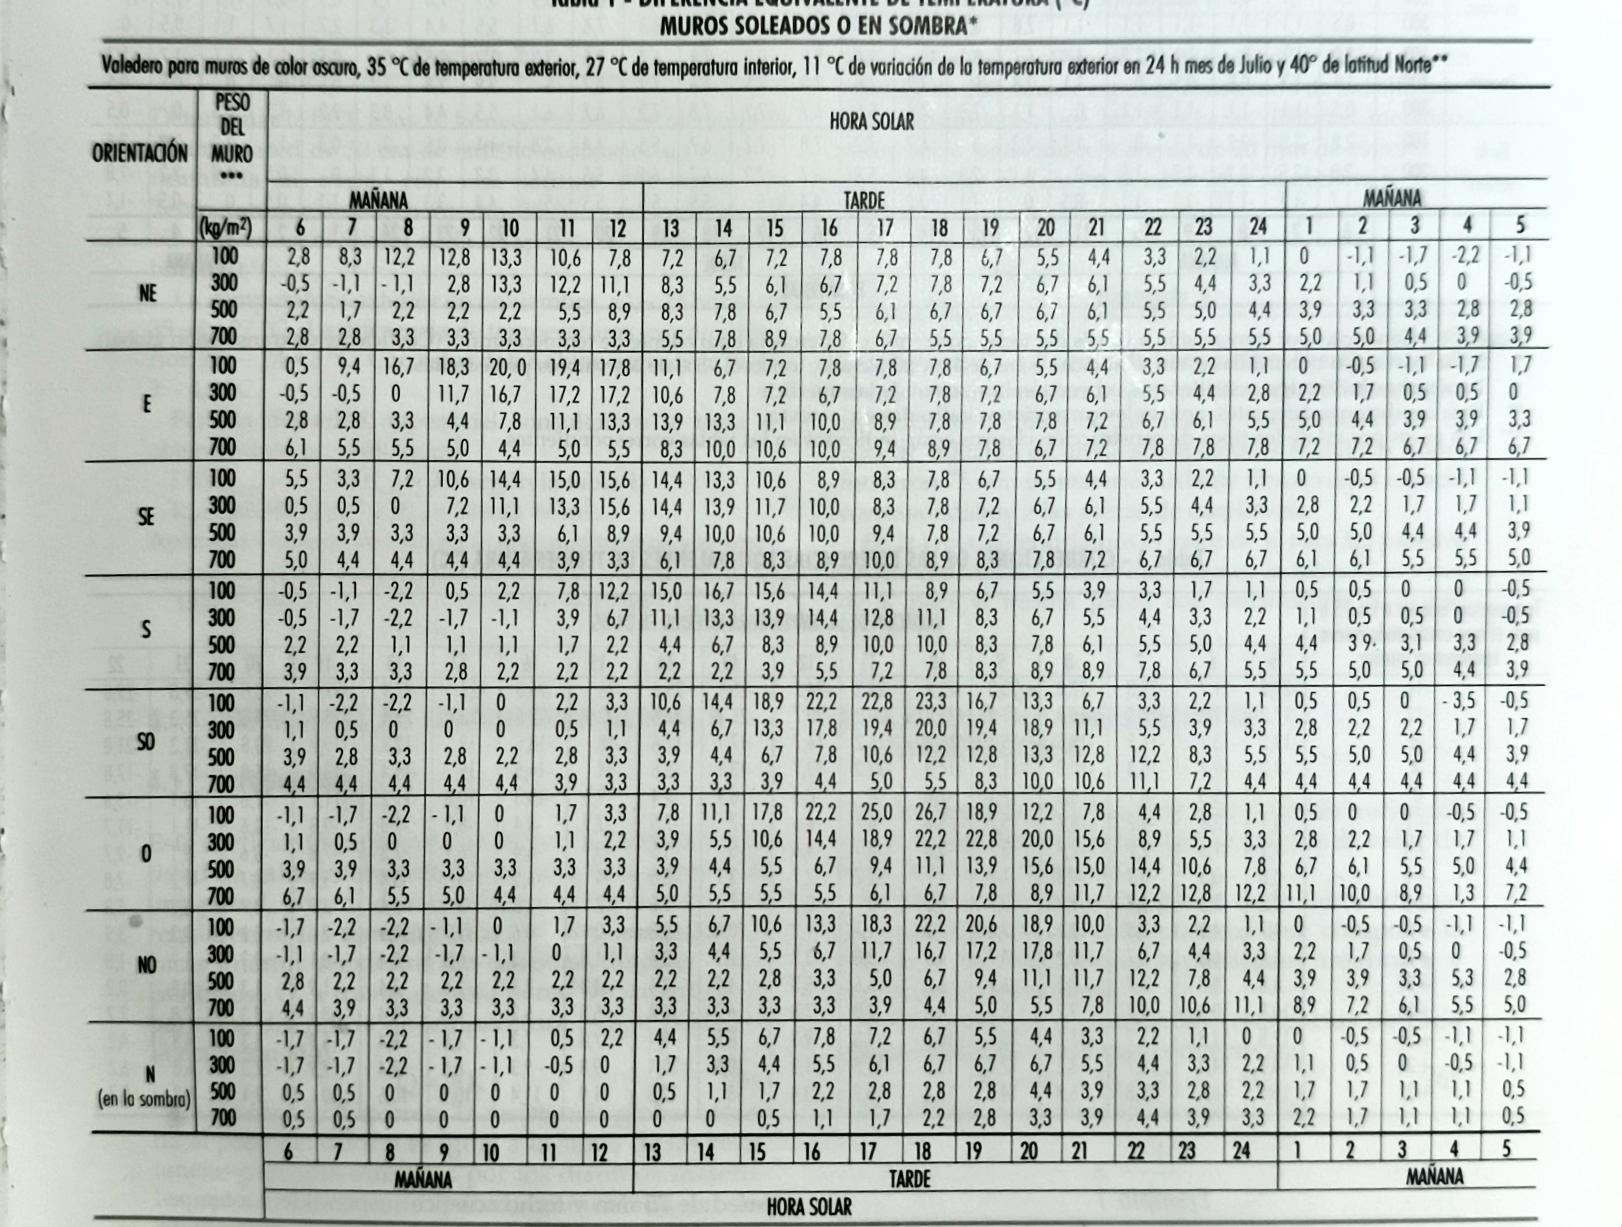
\includegraphics[width=0.8\linewidth]{calculo-termico/DET-muros.jpg}
\end{figure}
\begin{figure}[H]
	\centering
	\caption{Diferencia equivalente de temperatura para techos (\textcelsius)}
	\label{fig:DET-techos}
	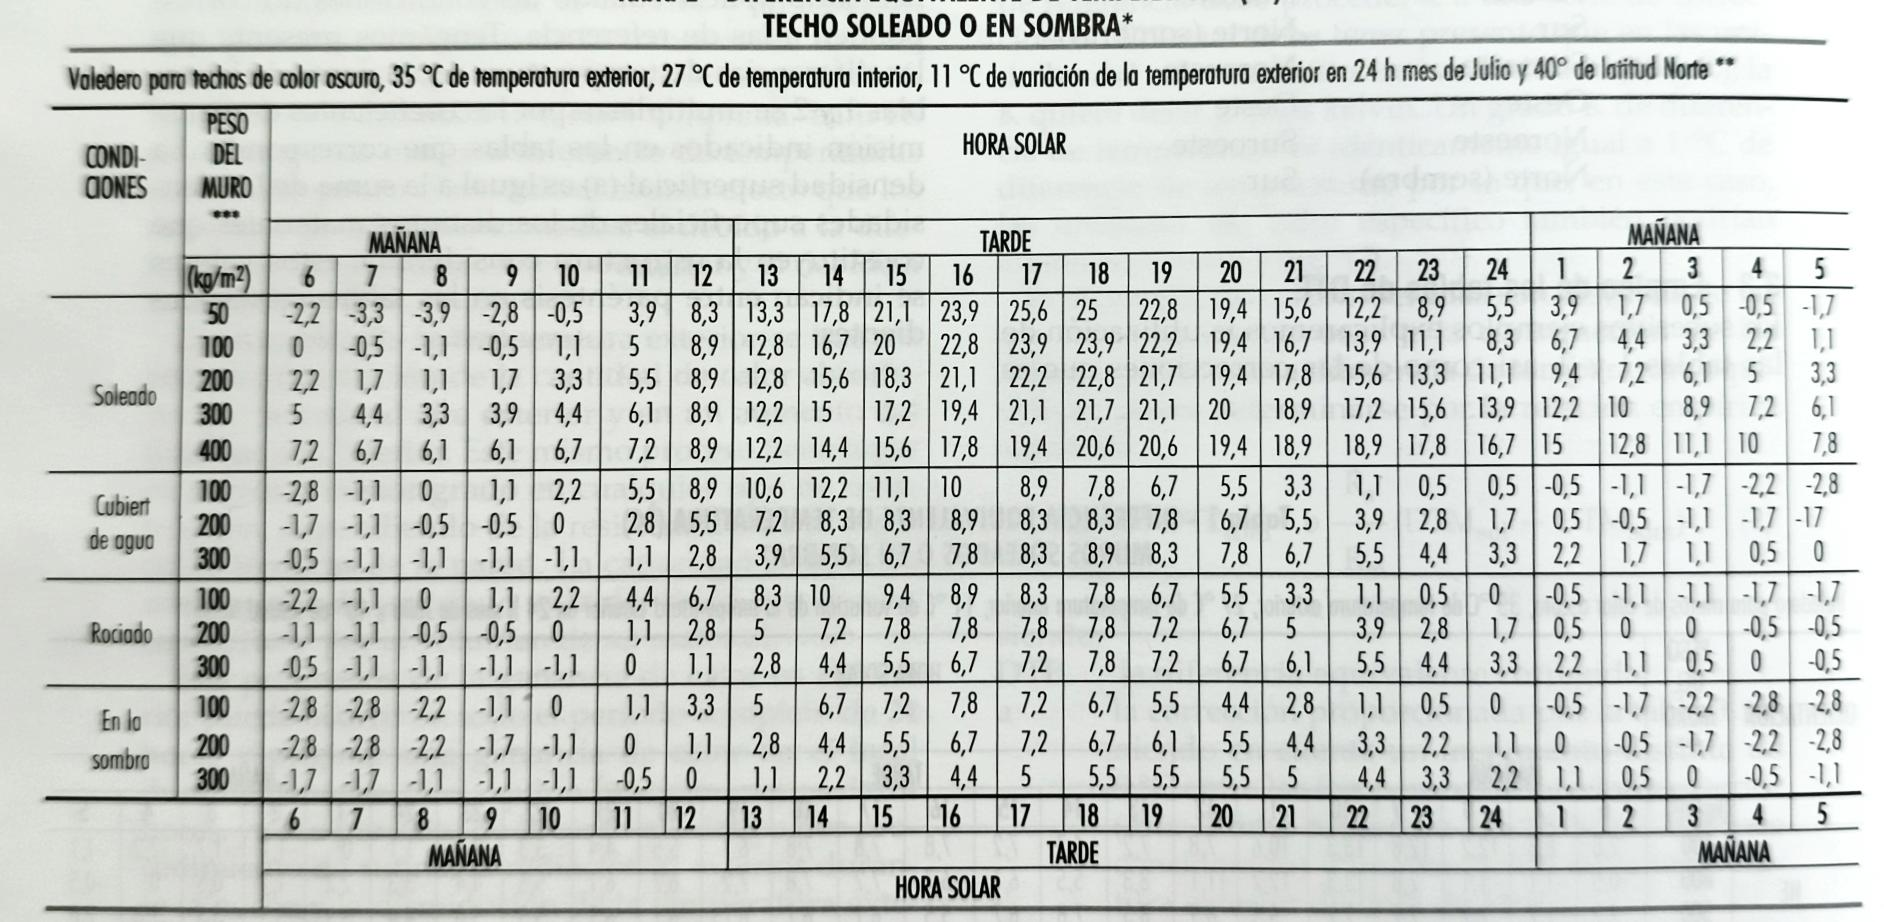
\includegraphics[width=0.8\linewidth]{calculo-termico/DET-techos.jpg}
\end{figure}
\begin{figure}[H]
	\centering
	\caption{Correcciones de las diferencias equivalentes de temperaturas (\textcelsius)}
	\label{fig:Correcion-DET}
	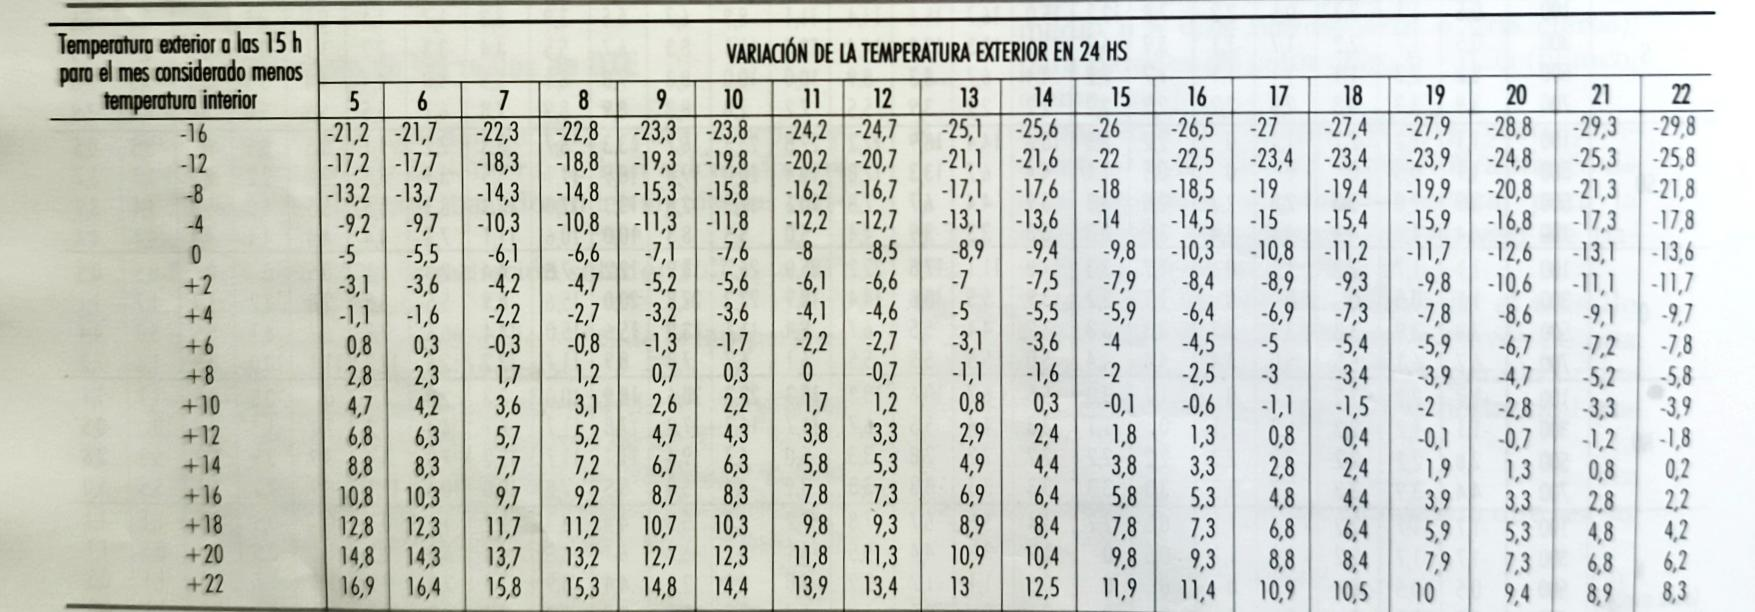
\includegraphics[width=0.8\linewidth]{calculo-termico/correccion-DET.jpg}
\end{figure}
% \ver{agregar tabla de temperatura equivalente del Carrier, si es que tiene}

\emph{Paredes y techos interiores}\\
Se trata de paredes y techos entre ambientes, por lo que en estos casos, no existe la radiación solar, pudiéndose considerar el salto térmico entre la temperatura de aire a ambos lados. De esa manera:

\begin{equation}\label{eq:transmision-interna}
	q_{Ti} = A \cdot k \cdot (t_e' - t_i)
\end{equation}

Donde\begin{itemize}
	\item $t_e'$ es la temperatura del aire del local vecino,
	\item $t_i$ es la temperatura del aire interior del ambiente.
\end{itemize}

Para cálculos prácticos \textcite{quadri2020} supone que un local no acondicionado se encuentra a una temperatura de alrededor de 3 °C menor que la temperatura de aire exterior.

\begin{equation}
	t_e' = t_e - 3\, \text{°C}
\end{equation}

La diferencia equivalente de temperatura para muros y techos interiores también puede obtenerse a partir de las tablas presentadas en la \autoref{fig:DET-muros} y la \autoref{fig:DET-techos} de \textcite{carrier2009}, según la hora solar. Dichos muros y techos se consideran en condiciones de sombra. 

\subsubsection{Ganancia de calor a través de ventanas}

La cantidad de calor que ingresa al sistema se da por transmisión y por radiación solar, entonces:
\begin{align}
	q_v &= q_{Tv} + q_{Rv}\\
	q_{Tv} &= A \cdot k \cdot (t_e - t_i)\\
	q_{Rv} &= A \cdot I \cdot c 
\end{align}
Donde \begin{itemize}
	\item $q_v$ es la ganancia de calor total del vidrio,
	\item $q_{Tv}$ es la ganancia por transmisión
	\item $q_{Rv}$ es la ganancia por radiación solar,
	\item $I$ es la intensidad de radiación solar,
	\item $c$ es el coeficiente de corrección por protección de ventana.
\end{itemize}       

En la Tabla 1 del capítulo 4 (pp. I-21 a I-26) del \citetitle{carrier2009}, se muestran los valores de \emph{intensidad de radiación solar} a través de vidrio sencillo. Por su parte, la Tabla 2 del mismo capítulo (pág. I-28) muestra  los \emph{coeficientes de corrección por protección de ventana}. 

Debe destacarse que el vidrio actúa como una \emph{trampa de calor}, dado que la radiación solar visible lo atraviesa, mientras que la radiación de calor no visible, como las emitidas en el interior de un local por los ocupantes no pasan al exterior. Este fenómeno se denomina \emph{efecto invernadero}, tal como se muestra en la \autoref{fig:efecto-invernadero}.

\begin{figure}
	\centering
	\caption{Pasaje de calor solar a través del vidrio}
	\label{fig:efecto-invernadero}
	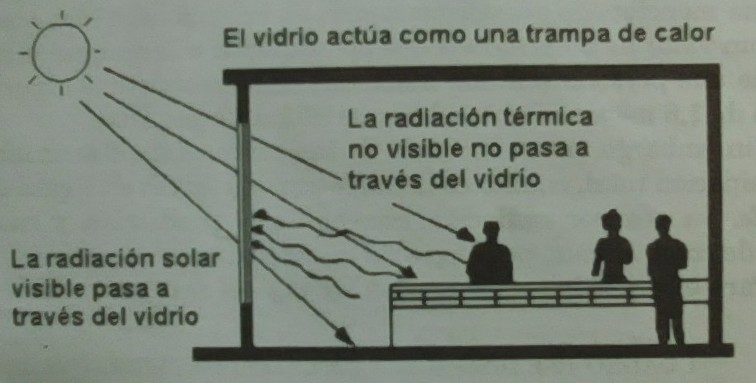
\includegraphics[width=0.6\linewidth]{calculo-termico/trampa-de-calor}
\end{figure}

\subsubsection{Ganancia de calor por aire exterior}
Es la ganancia (o p\'erdida) de calor debida al ingreso del aire exterior de manera voluntaria (ventilaci\'on) o involuntaria (infiltraci\'on), y tiene componente sensible y latente.

\emph{Infiltraci\'on}

Las infiltraciones ocurren por la velocidad del viento exterior que ejerce una presi\'on din\'amica sobre la fachada del edificio, produciendo un efecto de sobrepresi\'on exterior. Tambi\'en suelen darse las infiltraciones por el efecto chimenea o diferencia de densidades, esto ocurre por las diferencias de temperaturas entre el interior y exterior, lo que provoca una circulaci\'on natural del aire.

El caudal de aire de infiltraci\'on depende de la estanqueidad de las puertas y ventanas, la frecuencia de su uso, la porosidad de las paredes del edificio, de su altura, de si tiene o no escaleras o ascensores y, de la direcci\'on y velocidad del viento.

En el Cap\'itulo 6 del \citetitle{carrier2009} se muestran tablas para obtener el caudal de infiltraci\'on seg\'un el tipo de abertura, su frecuencia de utilizaci\'on o grado de apertura y su estanqueidad. Este caudal esta en m$^3$/h por m$^2$ de abertura, por lo tanto para obtener el caudal se debe multiplicar la superficie total del tipo de ventana o puerta de estudio. Las tablas fueron generadas para un viento de 12 km/h con una incidencia perpendicular a la abertura. En caso diferentes velocidades de viento se debe dividir la velocidad de viento real por 12 y luego multiplicar este valor por el obtenido en la tabla. Para direcciones oblicuas de viento con respecto a la superficie de la abertura se multiplica por 0,6 el valor obtenido en la tabla.

\emph{Ventilaci\'on}

Para evitar la sensaci\'on desagradable que produce el aire viciado es necesario introducir una cierta cantidad de aire exterior que se llama ventilaci\'on. En la pr\'actica, esta operaci\'on se hace filtrando y tratando t\'ermicamente el aire exterior para su posterior mezcla con el aire del local. La misma cantidad que se introduce se debe rechazar al exterior.

Según el \citetitle{carrier2009} de \textcite{carrier2009}, el caudal mínimo de ventilación se determina considerando el \citetitle{RITE} donde se obtienen las pautas que regulan la ventilaci\'on necesaria para cada espacio seg\'un el tipo de lugar y la actividad llevada en \'el. Se clasifican seg\'un el concepto de \emph{aire de óptima calidad} (IDA), que distingue los siguientes niveles de calidad:
\begin{itemize}
	\item IDA 1 - Aire de \'optima calidad: hospitales, cl\'inicas, laboratorios y guarder\'ias.
	\item IDA 2 - Aire de buena calidad: oficinas, residencias, salas de lectura, museos y similares.
	\item IDA 3 - Aire de media calidad: edificios comerciales, cines, teatros, restaurantes, cafeter\'ias y similares.
	\item IDA 4 - Aire de calidad baja.
\end{itemize}
En funci\'on del IDA, con la \autoref{tab:caudales-aire-exterior-por-persona} se puede hallar el caudal de aire de ventilaci\'on por persona. Multiplicando por la cantidad de personas totales que estar\'an en el local se obtiene el caudal de ventilaci\'on necesario.
\begin{figure}
    \centering
    \caption{Caudales de aire exterior en l/s}
    \label{fig:caudales-aire-exterior-por-persona}
    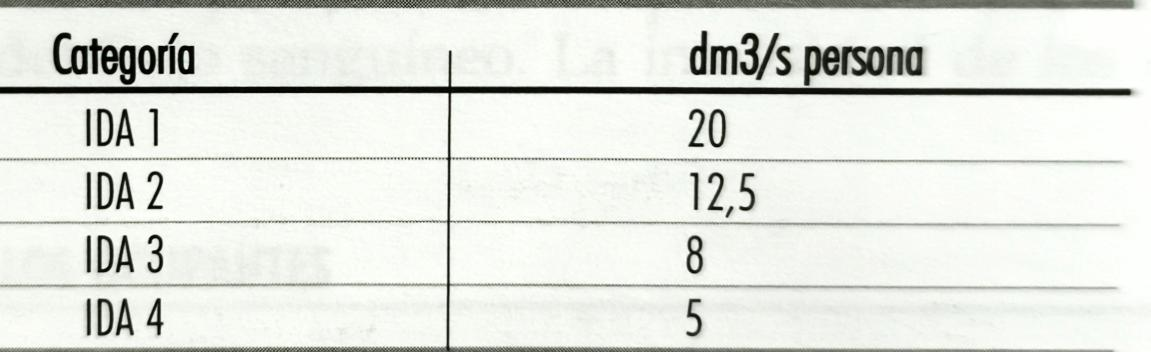
\includegraphics[width=0.6\linewidth]{calculo-termico/caudales-aire-exterior-por-persona.jpg}

\end{figure}

\begin{table}[h]
	\centering\caption{Caudales de aire exterior en l/s}
	\label{tab:caudales-aire-exterior-por-persona}
	\begin{tabular}{ll}
		\hline
		Categoría 1 & dm3/s persona \\ \hline
		IDA 1    & 20    \\ \hline
		IDA 2    & 12.5    \\ \hline
		IDA 3    & 8    \\ \hline
		IDA 4    & 5    \\ \hline
	\end{tabular}
\end{table}

Los valores indicados en la \autoref{tab:caudales-aire-exterior-por-persona} corresponden a situaciones en las que las personas tengan una actividad metab\'olica de alrededor de 1,2 met. El met es una unidad metab\'olica equivalente a 58,2 W/m$^2$.

Por otro lado, en el libro \citetitle{quadri2020} de \textcite{quadri2020} se presenta un enfoque similar, donde considera el caudal de aire exterior a ingresar como un porcentaje del caudal de aire de circulación. Este último se calcula como:
\begin{equation}
	\label{eq:caudal-de-circulacion}
	C = \dfrac{Q_{si}}{17 \cdot (t_i - t_I)}
\end{equation}
Siendo
\begin{itemize}
	\item $C$ el caudal de aire en circulación (m$^3$/min),
	\item $Q_{si}$ la ganancia de calor sensible total del local (kcal/h), expuesta en la \autoref{sec:balance-verano},
	\item $t_i$ la temperatura del aire del ambiente (°C),
	\item $t_I$ la temperatura de impulsión al local (°C),
	\item $17$ valor que se considera constante.
\end{itemize}

En la práctica, la \emph{temperatura de impulsión del aire puede estimarse en 10 °C menor que la temperatura de diseño del local}, por lo que el salto térmico puede tomarse de 10 °C. Sin embargo, para cálculos más precisos, la temperatura de impulsión se obtiene en función del tipo de evaporador utilizado y a partir del diagrama psicrométrico. 


Entonces, el caudal de aire exterior que debe ingresar es:
\begin{equation}
	C_{ae} = a \cdot C
\end{equation}
Donde
\begin{itemize}
	\item $C_{ae}$ es el caudal de aire nuevo exterior,
	\item $a$ es el porcentaje de aire nuevo,
	\item $C$ es el caudal de aire en circulación.
\end{itemize}

Aunque depende de la aplicación, generalmente, para locales con muchas personas se toma un porcentaje entre un 25 y 30\%, para edificios de oficinas entre el 15 y el 25\% y para edificios de viviendas del 10 al 20\%.

Siempre es necesario verificar si se cumple con el aire de ventilación mínimo que se establece reglamentariamente. En la \autoref{tab:requerimientos-aire} \parencite{quadri2020}, se indican las cantidades mínimas recomendadas para diversas aplicaciones.

\begin{table}[h]
	\centering
	\caption{Requerimientos de aire nuevo mínimos.}
	\label{tab:requerimientos-aire}
	\begin{tabular}{lc}
		\hline
		Aplicaciones & m$^3$/min pers \\
		\hline
		Lugares de trabajo en general & $0.5$ \\
		Oficinas generales & $0.5$ \\
		Oficinas privadas & $0.6$ \\
		Restaurantes y lugares afines (con personas fumando) & $0.8$ \\
		Oficinas privadas (con personas fumando) & $0.8$ \\
		Viviendas & $0.5$ \\
		Teatros, cines, auditorios & $0.6$ \\
		\hline
	\end{tabular}
\end{table}

\textcite{quadri2020} establece que la ganancia total de calor debida al aire exterior $Q_{Te}$ son del tipo sensible del aire seco y latente en forma de vapor de agua.

\begin{equation}\label{eq:calor-aire-exterior}
	Q_{Te} = Q_{se} + Q_{le}
\end{equation}

El \emph{calor sensible del aire seco} se calcula como:
\begin{equation}
	Q_{se} = 17 \cdot C_{ae} \cdot (t_e - t_i)
\end{equation}
Donde
\begin{itemize}
	\item $Q_{se}$ es el calor sensible del aire exterior (kcal/h),
	\item $C_{ae}$ es el caudal del aire exterior (m$^3$/min),
	\item $t_i$ es la temperatura del aire del ambiente (°C),
	\item $t_e$ es la temperatura del aire exterior (°C),
	\item $17$ es un valor constante.
\end{itemize}

El \emph{calor latente del vapor de agua} se determina como:
\begin{equation}
	Q_{le} = 42 \cdot C_{ae} \cdot (\omega_e - \omega_i) 
\end{equation}
Donde \begin{itemize}
	\item $Q_{le}$ es el calor latente del vapor de agua del aire exterior (kcal/h),
	\item $C_{ae}$ es el caudal del aire exterior (m$^3$/min),
	\item $\omega_i$ es la humedad absoluta del aire del ambiente (gr/kg),
	\item $\omega_e$ es la humedad absoluta del aire exterior (gr/kg),
	\item $42$ es un valor constante.
\end{itemize}

\subsection{Cargas internas}

\subsubsection{Ganancia de calor de las personas}
La cantidad de calor cedido por una persona depende del grado de actividad y de la temperatura ambiente. Los valores de la Tabla de la \autoref{fig:calor-ocupantes} se basan en la cantidad media de calor generado por un hombre adulto de $68$ kg de peso para distintas actividades y con una permanencia superior a tres horas en el local.

\begin{figure}[H]
	\centering
	\caption{Ganancia de calor debida a los ocupantes, según datos de la Tabla 1 del Capítulo 7 en el \citetitle{carrier2009}.}
	\label{fig:calor-ocupantes}
	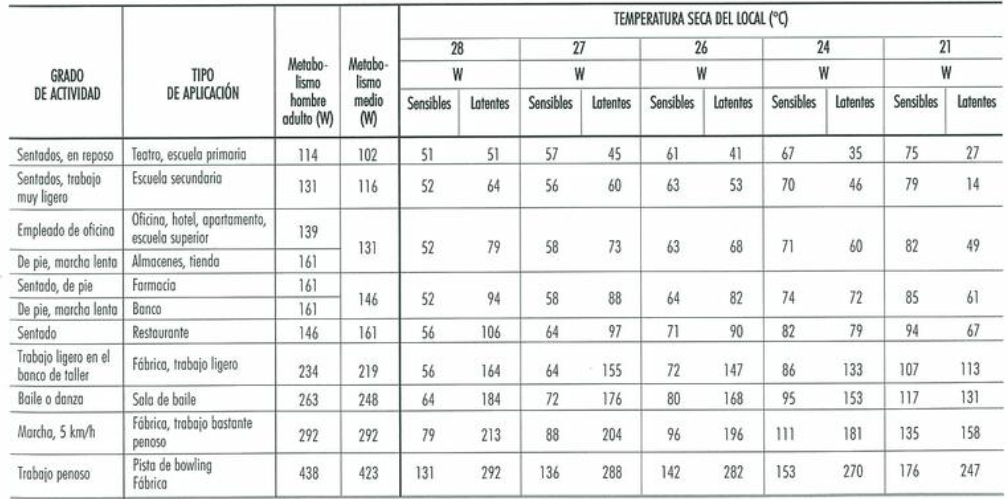
\includegraphics[width=\linewidth]{calculo-termico/calor-ocupantes.png}
\end{figure}


Aumentando el grado de actividad se incrementa la cantidad de calor latente disipado, debido a la evaporación del cuerpo.

\subsubsection{Ganancia de calor de la iluminación}

El calor proveniente de la iluminación es totalmente sensible. El calor sensible liberado por cada luminaria corresponde al 90\% de la potencia consumida para lámparas incandescentes, 75\% para tubos fluorescentes y menos del 30\% para lámparas leds.

\subsubsection{Ganancia de calor de diversos aparatos}

La carga debida a los aparatos es sensible y latente, dependiendo de su función. En \citetitle[Capítulo 7]{carrier2009}, las Tablas 2 a 4 muestran las cargas debidas a aparatos en restaurantes y a diversos aparatos, respectivamente.

Para motores eléctricos, el calor sensible disipado se calcula como la diferencia entre la potencia eléctrica consumida y la potencia útil:
\begin{equation}
	q_m = P_e (1-\eta)
\end{equation}
Siendo
\begin{itemize}
	\item $q_m$ la potencia térmica disipada,
	\item $P_e$ la potencia eléctrica consumida,
	\item $\eta$ el rendimiento del motor.
\end{itemize}

\citeauthor{carrier2009} considera que la carga depende de la ubicación del motor y de la máquina accionada, por lo que pueden darse tres casos:
\begin{enumerate}
	\item El motor está situado dentro del espacio acondicionado y la máquina está fuera, el aporte estará dado por $q_m$.
	\item La máquina está dentro del espacio y el motor fuera, el aporte será $P_e \cdot \eta$
	\item Ambos, motor y máquina están dentro del espacio, el aporte será $P_e$.
\end{enumerate}
El rendimiento del motor viene dado por las características y está dado por el fabricante. Si no se conoce, puede utilizarse los valores de la \autoref{tab:rendimiento-motor} extraídos de la bibliografía.

\begin{table}[h]
	\centering
	\caption{Rendimiento aproximado de motores eléctricos de jaula de ardilla.}
	\label{tab:rendimiento-motor}
	\begin{tabular}{c*{9}{>{\centering\arraybackslash}p{1cm}}}
		\hline
		Potencia kW & 0,05 & 0,1 & 0,5 & 1 & 5 & 15 & 30 & 50 & 90 \\
		\hline
		Eficiencia \% & 50 & 60 & 70 & 83 & 88 & 92 & 93 & 94 & 95 \\
		\hline
	\end{tabular}
\end{table}
\subsection{Cargas debido a la instalación}
:) Capítulo 7 de carrier, o y habíamos puesto esto?

\section{Balance térmico en verano}\label{sec:balance-verano}
La carga de refrigeración es el calor que se debe eliminar del sistema para mantener las condiciones internas del diseño. 

Como indica \textcite{quadri2020}, la ganancia de calor total del interno del local se calcula como
\begin{equation}
	Q_{Ti} = Q_{si} + Q_{li}
\end{equation}
Donde
\begin{itemize}
	\item $Q_{Ti}$ es la ganancia total de calor del local,
	\item $Q_{si}$ es la ganancia total de calor sensible del local,
	\item $Q_{li}$ es la ganancia total de calor latente del local.
\end{itemize}

En verano, la carga térmica total del local se determina como la suma de los aportes de calor generados por cada una de las cargas externas por transmisión. Las cargas internas incluyen las debidas a los ocupantes y los dispositivos varios, mientras que las externas son las debidas a la transmisión y radiación de calor.

\subsection{Carga total de refrigeración}

La carga total de refrigeración $Q_{Tr}$ que requiere el equipo de aire acondicionado será igual a:
\begin{equation}
	Q_{Tr} = Q_{Ti} + Q_{Te}
\end{equation}

Siendo $Q_{Ti}$ la carga total interna y $Q_{Te}$ la carga total debido al aire exterior calculada según la \autoref{eq:calor-aire-exterior}.

\section{Balance térmico en invierno}

La carga de calefacción es el calor que se debe suministrar al sistema para mantener las condiciones internas del diseño.

En el balance térmico en invierno no se consideran los aportes de calor generados por personas, iluminación, la radiación solar, etc., ya que estos benefician al sistema. El cálculo se realiza contemplando la condición más desfavorable, es decir, el momento en que el equipo de climatización debe suministrar la mayor cantidad de calor.

La carga total de calefacción $Q_{Tc}$ es:
\begin{equation}
	Q_{Tc} = Q_{si} + Q_{se}
\end{equation}
Donde $Q_{si}$ es la pérdida de calor sensible total del local por transmisión y $Q_{se}$ es la pérdida de calor debida al aire frío exterior.

La cantidad total de calor sensible que pierde el local se calcula como
\begin{equation}\label{eq_calor-sensible-invierno}
	Q_{si} = Q_o \cdot (1 + Z_d + Z_h + Z_c)
\end{equation}
Donde
\begin{itemize}
	\item $Q_o$ es la pérdida por transmisión de las superficies del ambiente,
	\item $Z_d$ factor por la interrupción del servicio,
	\item $Z_h$ factor por orientación,
	\item $Z_c$ factor por pérdidas en cañerías o conductos.
\end{itemize}

La pérdida de calor por transmisión $Q_o$ se calcula como la suma de todas las pérdidas individuales de cada una de las superficies del local.
\begin{equation}
	Q_o = \sum q_o
\end{equation}
Donde $q_o$ se calcula según las ecuaciones \ref{eq:transmision} y \ref{eq:transmision-interna}.

La \autoref{tab:factores-suplementos} expone un resumen de los valores de los factores por modificación que intervienen en la \autoref{eq_calor-sensible-invierno}.

\begin{table}[h]
	\centering
	\caption{poner un caption :c}
	\label{tab:factores-suplementos}
	\begin{tabular}{*{2}{p{5cm}} c}
		\hline
		\multicolumn{2}{l}{Suplemento por interrupción de servicio} & $Z_d$ \\ \hline
		Servicio ininterrumpido con marcha reducida en la noche   & Viviendas, hospitales, asilos, etc.   & $0.07$   \\ 
		Interrumpido de 8 a 12 h   & Comercio, oficinas, etc.   & $0.15$   \\ 
		Interrumpido de 12 a 16 h   & Funcionamiento circunstancial   & $0.25$  \\ \hline
		\multicolumn{2}{l}{Suplemento por orientación} & $Z_h$ \\ \hline
		E y O & & $0$\\
		N, NE y NO && $-0.05$ \\
		S, SE y SO && $0.05$\\\hline
		\multicolumn{2}{l}{Suplemento por pérdidas de calor en conductos} & $Z_c = 0.1$\\\hline
	\end{tabular}
\end{table}

\subsection{Diferencia entre temporadas de refrigeraci\'on y de calefacci\'on}

Durante la temporada de calefacción, es común que la humedad absoluta del aire exterior es mucho menor que la del interior. Como siempre existe cierta renovación de aire, esto provoca una pérdida continua de vapor de agua en el ambiente acondicionado. Esto puede ser una ayuda si las cargas interiores generan cierto vapor de agua y se mantiene una humedad relativa agradable, en caso contrario, deber\'a suministrarse vapor de agua.
